\documentclass[12pt,addpoints]{exam}
\usepackage[utf8]{inputenc}
\usepackage[T1]{fontenc}
\usepackage[brazil]{babel}
\usepackage[a4paper, margin=2cm]{geometry}
\usepackage{graphicx, amsmath, amsfonts, amssymb, xcolor, url, tikz, pgfplots, subfigure}

\newcommand{\disciplina}{Laboratório de Princípios de Comunicações}
\newcommand{\periodo}{2020.1}
\newcommand{\avaliacao}{Guia de Experimentos 5}
\newcommand{\tema}{Comunicações digitais.}
%\newcommand{\professor}{Leocarlos B.\ S.\ Lima e Edson P.\ da Silva}
\newcommand{\professor}{Edson P.\ da Silva e Luciana Veloso}
%\newcommand{\professor}{Edmar C. Gurjão e Luciana Veloso}
%\newcommand{\professor}{Bruno\ B.\ Albert e Edson P.\ da Silva}

\pagestyle{head}
\firstpageheader{}{}{}
\runningheader{Lab.\ Princ.\ Comunicações}{\avaliacao}{Página \thepage}
\runningheadrule
\pointpoints{ponto}{pontos}
\newtheorem{exemplo}{Exemplo}[section]

\begin{document}
    
\noindent 
\includegraphics[height=2cm]{../Figuras/UFCGLogo.png} \hfill
\begin{minipage}{.66\textwidth} \large \centering \vspace{-1.8cm}
    Universidade Federal de Campina Grande -- UFCG \\
    Unidade Acadêmica de Engenharia Elétrica -- UAEE \\
    Curso de Graduação em Engenharia Elétrica
\end{minipage}
\hfill 
\includegraphics[height=2cm]{../Figuras/DEELogo.png} \\[12pt]

\noindent
\begin{tabular*}{\textwidth}{l @{\extracolsep{\fill}} r @{\extracolsep{6pt}} l}
    \textbf{\disciplina} && \\
    Período \periodo && \\
    \textbf{\avaliacao} && \\
    Tema(s): \tema && \\
    Professor(es): \professor && \\
\end{tabular*}
\noindent\rule[2ex]{\textwidth}{2pt}
    
\section{Introdução}

O presente guia descreve atividades experimentais a serem realizadas na disciplina Laboratório de Princípios de Comunicações do curso de graduação em Engenharia Elétrica da Universidade Federal de Campina Grande -- UFCG.

Os experimentos propostos deverão ser realizados no Laboratório de Princípios de Comunicações -- LPC, localizado na Central de Laboratórios da Unidade Acadêmica de Engenharia Elétrica da UFCG, empregando:
\begin{itemize}
    \item Computador com software GNU Radio Companion -- GRC (\url{http://gnuradio.org/}) instalado;
    \item Módulo USRP (do inglês \textit{Universal Software Radio Peripheral}) para transmissão e recepção de sinais numa abordagem conhecida como Rádio Definido por Software -- RDS.
\end{itemize}

Na seção \ref{sect:Preparacao} deste guia, propõe-se um conjunto de atividades de preparação a serem desenvolvidas pelo aluno antes da aula em que serão realizadas as práticas experimentais. Sem a realização prévia destas atividades pelo aluno, as práticas experimentais propostas ficarão comprometidas, tanto no tempo necessário para sua realização quanto no aproveitamento pelo aluno. Por essa razão, \textbf{o aluno só poderá realizar os experimentos em laboratório se apresentar ao professor no início da aula os resultados da preparação proposta}. 

A aula terá duração de duas horas e o aluno deverá entregar ao seu término, por escrito, respostas às questões referentes aos experimentos realizados propostas na Folha de Respostas (parte final do guia).

\section{Objetivos}

As práticas experimentais aqui propostas têm por objetivos:
\begin{itemize}
    \item Analisar diagrama de olho de sinal digital;
    \item Projetar e analisar equalizador de canal e seu efeito sobre o sinal recebido;
    \item Observar emprego de código duobinário sobre sinal transmitido;
    \item Observar efeito de ruído de canal em BER e SNR em sinal modulado digital transmitido.
\end{itemize}

\section{Preparação} \label{sect:Preparacao}

\subsection{Estudo}

Revise e pesquise sobre os conceitos:
\begin{itemize}
    \item Diagrama de olho;
    \item Equalizador de zero forçado (\textit{zero-forcing equalizer});
    \item Código duobinário;
    \item Modulações M-PAM e M-QAM.
\end{itemize}

\subsection{Estudo de caso: compensação da dispersão cromática em fibras ópticas}
Em óptica, a dispersão é o fenômeno que ocorre em meios no quais a velocidade de fase de uma onda propagante depende de sua frequência. Meios com essa propriedade são conhecidos como meios dispersivos. Algumas vezes o termo \textit{dispersão cromática} é usado para melhor definir a origem do fenômeno. Embora o conceito seja comumente vinculado à óptica, fenômenos similares pode ocorrer em qualquer tipo de propagação de onda, como é o caso da dispersão acústica de ondas sonoras.
 
Uma consequência óptica importante e familiar da dispersão é a mudança no ângulo de refração de diferentes cores (componentes de frequência) de luz, como visto no espectro produzido por um prisma dispersivo e na aberração cromática de lentes. O exemplo mais conhecido de dispersão é provavelmente um arco-íris, no qual a dispersão causa a separação espacial de uma luz branca em componentes de diferentes comprimentos de onda (cores diferentes). 

Por sua vez, em sistemas de comunicações via fibra óptica, a dispersão cromática faz com que pulsos transmitidos pela fibra se espalhem no tempo, causando interferência entre símbolos e degradando os sinais em longas distâncias de transmissão. O efeito da dispersão cromática numa sequência de pulsos transmitidos por uma fibra óptica está ilustrado na Fig.~\ref{fig:GRC_5-0}. Perceba que a dispersão é caracterizada pelo alargamento temporal dos pulsos transmitidos, bem como a diminuição da potência de pico do sinal. Num sistema de comunicações, pulsos diferentes carregam informações  distintas (\textit{bits} distintos) e a interferência entre eles pode causar erros na recepção da informação, podendo até inviabilizar a comunicação.

Numa fibra óptica, diversos tipos de dispersão cromática podem acontecer. Entretanto, a dispersão de segunda ordem é a mais importante, por gerar a maior contribuição para a interferência entre símbolos nos sinais de comunicação. 

\begin{figure}[h]
        \centering
        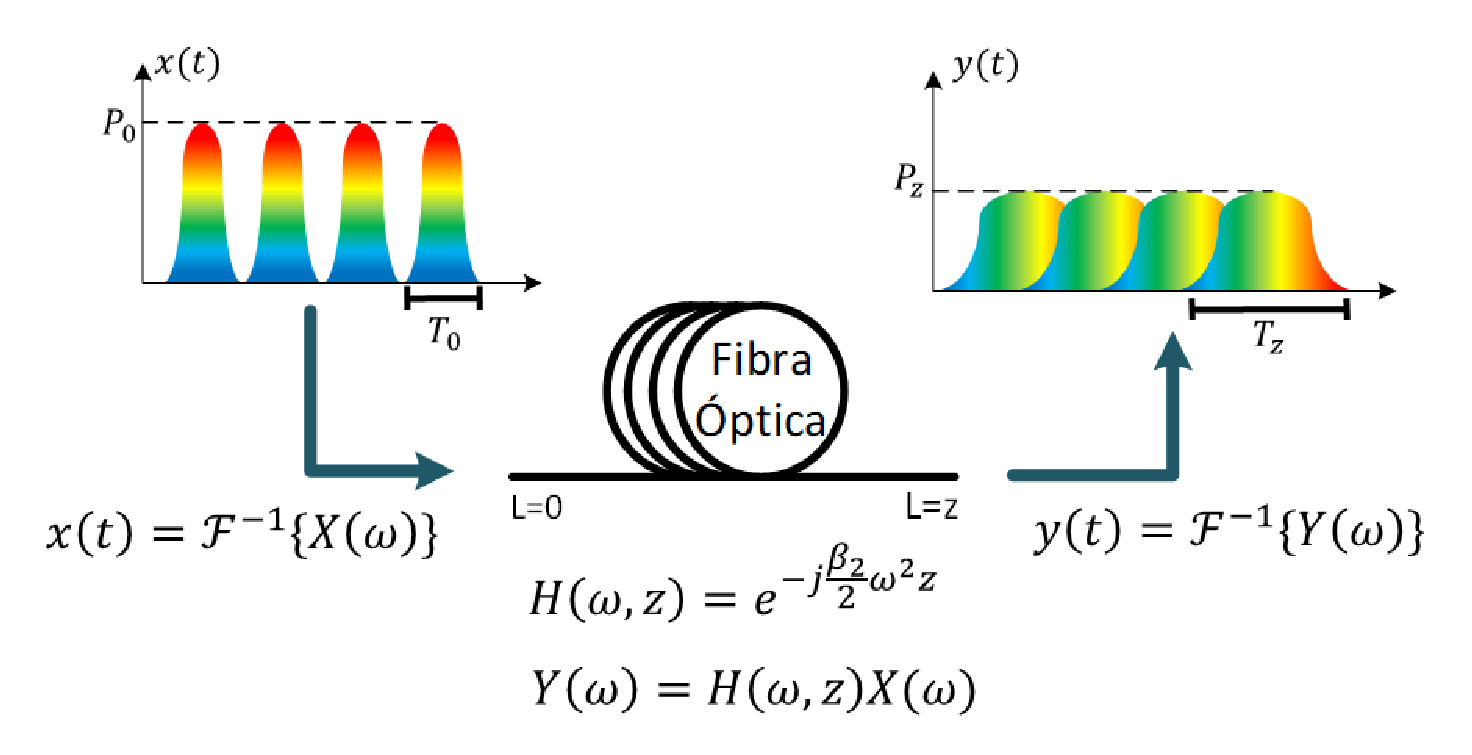
\includegraphics[width=0.75\textwidth]{Figuras/Labo5-0}
        \caption{Modelo no domínio da frequência de uma fibra óptica em que os sinais propagantes estão sujeitos apenas ao fenômeno da dispersão cromática de segunda ordem.}
        \label{fig:GRC_5-0}
\end{figure}

Se considerarmos que apenas a dispersão cromática de segunda ordem ocorre na fibra, podemos modelar o efeito da propagação do sinal pelo guia de acordo com a resposta em frequência definida na Eq.~\ref{CDtf}:
\begin{equation}\label{CDtf}
    H(\omega, z) = e^{-j\frac{\beta_2}{2}\omega^2z},
\end{equation}
\noindent em que $z$ é a distância de propagação do sinal e $\beta_2$ é o parâmetro que caracteriza a dispersão de segunda ordem e que depende da fibra utilizada na trasmissão. Note em \ref{CDtf} que o efeito da dispersão no sinal transmitido dependerá de suas componentes de frequência e de sua distância de propagação.

Felizmente, devido à linearidade do fenômeno, os efeitos da dispersão cromática podem ser revertidos com o uso de equalizadores de zero forçados (\textit{zero-forcing equalizers}). Tais equalizadores podem ser implementados tanto no domínio óptico, via fibras compensadoras de dispersão (\textit{dispersion compensating fibers -- DCF's}), ou no domínio digital, como por equalizadores baseados em filtros digitais. Sem estes equalizadores, as altas taxas de transmissão de bits alcançadas nos dias atuais em cabos ópticos submarinos tornariam-se inviáveis, dificultando a expansão da Internet até o seu estado atual.

Considerando o modelo de resposta em frequência definido na Eq.~\ref{CDtf}, a resposta em frequência do equalizador de zero forçado será expressa por
\begin{equation}\label{CDzf}
H_{ZF}(\omega, z) = \frac{1}{H(\omega, z)}= \frac{1}{e^{-j\frac{\beta_2}{2}\omega^2z}} = e^{j\frac{\beta_2}{2}\omega^2z}
\end{equation}

Fazendo a transformada de Fourier inversa de $H_{ZF}(\omega, z)$, obtém-se a resposta ao impulso $h_{ZF}(t, z)$ do filtro equalizador que, posteriormente, pode ser aproximada por um filtro digital $h_{ZF}(kT, z)$ de resposta ao impulso finita (\textit{finite impulse response -- FIR}).

\subsection{Problemas}

Os problemas propostos a seguir devem ser obrigatoriamente resolvidos e apresentados por escrito ao professor antes do início das práticas de laboratório. Os resultados destes problemas serão necessários para a realização dos experimentos propostos. 

\begin{enumerate}
    \item Que condição $H(\omega, z)$ deve satisfazer para que seja possível definir o equalizador de zero forçado $H_{ZF}(\omega, z)$ como expresso na Eq.~\ref{CDzf}? Essa condição é satisfeita para o modelo da dispersão cromática descrito na Eq.~\ref{CDtf}?
    \item Utilizando o código \textbf{Exp5.m} fornecido pelo professor, use o MATLAB/OCTAVE para calcular os coeficientes do filtros FIR que modelam a dispersão cromática e o equalizador de zero forçado para as seguintes distâncias:
    \begin{parts}
        \part $z_1$ = 1500~km  
        \part $z_2$ = 3000~km
        \part $z_3$ = 4000~km
        \part $z_4$ = 8000~km
    \end{parts}
    Os coeficientes dos filtros FIR projetados (i.e., a saída MATLAB/OCTAVE) serão salvos num arquivo \textbf{.TXT}. Estes coeficientes serão utilizados no experimento.
    \item De que forma é possível utilizar o mesmo filtro equalizador projetado para $z_3$ para equalizar $z_4$? (Dica: analise as Eq.~\ref{CDtf} e \ref{CDzf}))
\end{enumerate}

\section{Experimentos}

A seguir são descritas práticas experimentais a serem realizadas pelo aluno em aula de laboratório. 

\subsection{Experimento 1 -- Diagrama de olho}

O objetivo deste experimento é identificar os elementos de um diagrama de olho de um sinal 2-PAM e observar seu comportamento mediante adição de ruído.

\begin{enumerate}
    \item Antes de iniciar as atividades com o GRC, crie uma pasta para guardar os arquivos de seus experimentos e copie nela os modelos de diagrama (arquivos .GRC) disponibilizados pelo professor para esta aula. \textbf{Não deixe de realizar isso, pois o computador deste laboratório não é para seu uso pessoal e os arquivos que você utilizará serão alterados por você durante o experimento};
    \item Execute o software GRC e abra o arquivo \textbf{Labo5-1.grc}. A Figura \ref{fig:GRC_5-1} ilustra o diagrama deste experimento. Ele consiste na transmissão de um sinal 2-PAM e recepção do mesmo acrescido de ruído de canal. O gráfico apresentado permite observar o diagrama de olho construído a partir da parte real do sinal recebido;
    \item Para conseguir visualizar o diagrama de olho, marque a opção \textbf{Persistence} no canto superior do painel, à direita do gráfico, ajuste o valor \textbf{Analog Alpha} (pequena régua deslizante que surge sob a opção \textbf{Persistence}) para seu valor mínimo (0.01000) e aguarde a transmissão de vários pulsos para que o diagrama de olho seja desenhado. 
    \item Um régua deslizante localizada sob o painel do diagrama de olho permite alterar a potência do ruído de canal e observar seu efeito sobre o diagrama de olho e sobre a relação sinal-ruído (SNR) no sinal recebido. Após alterar o nível de ruído, desmarque a opção \textbf{Persistence} para limpar o gráfico e volte a marcá-la para que novo diagrama de olho seja desenhado para o novo nível de ruído;
    \begin{figure}[htb]
        \centering
        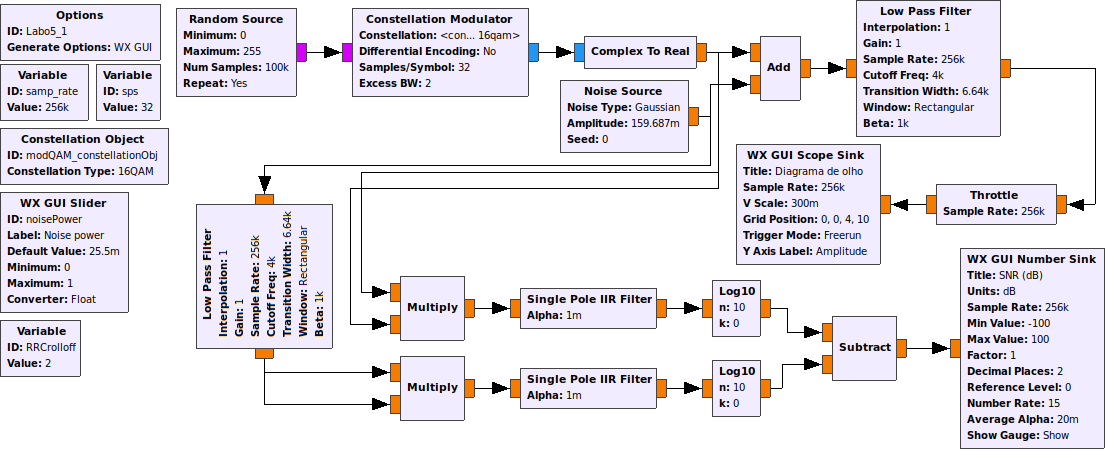
\includegraphics[width=\textwidth]{Figuras/Labo5-1}
        \caption{Diagrama de blocos para análise de diagrama de olho de sinal 2-PAM.}
        \label{fig:GRC_5-1}
    \end{figure}
  \item Execute o diagrama e responda às questões propostas na Folha de Respostas.
\end{enumerate}

\subsection{Experimento 2 -- Equalização}

O objetivo deste experimento é analisar o emprego de equalizador de zero forçado para minimizar a interferência intersimbólica observada através de diagrama de olho de sinal recebido após o sinal trafegar por canal com resposta $H(\omega, z) = e^{-j\frac{\beta_2}{2} \omega^2z}$ (dispersão cromática no canal óptico).

\begin{enumerate}
    \item Abra o arquivo \textbf{Labo5-2.grc} disponibilizado pelo professor. A Figura \ref{fig:GRC_5-2} ilustra o diagrama deste experimento. Uma modulação 4-PAM é empregada e três diagramas de olho são apresentados: 
    \begin{itemize}
        \item um do sinal transmitido, portanto sem distorção de canal, em azul;
        \item um do sinal recebido não equalizado, portanto distorcido pelo canal, em verde, e;
        \item um do sinal recebido e equalizado, em vermelho.
    \end{itemize}
    \begin{figure}[htb]
        \centering
        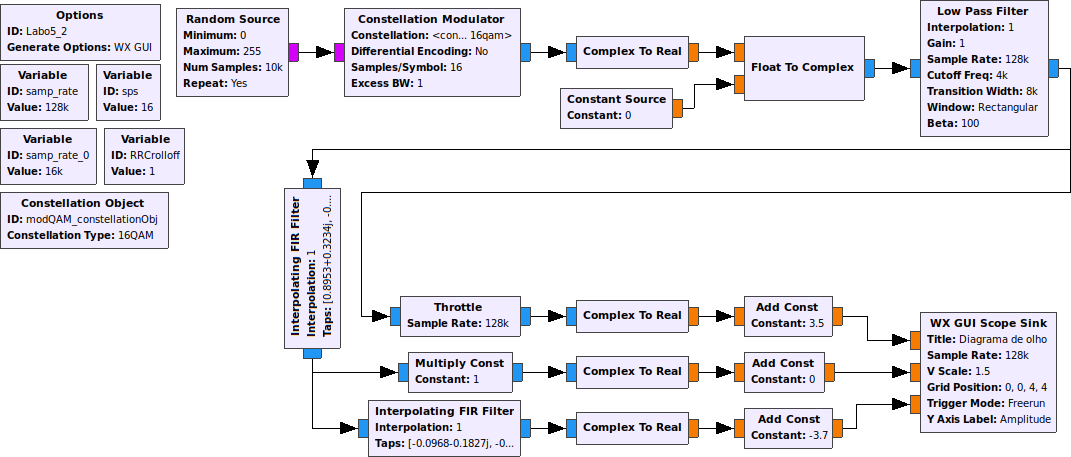
\includegraphics[width=\textwidth]{Figuras/Labo5-2}
        \caption{Diagrama de blocos ilustrando a aplicação de um equalizador de zero forçado para compensação da dispersão cromática da fibra óptica.}
        \label{fig:GRC_5-2}
    \end{figure}
    \item Introduza no bloco \textbf{Interpolating FIR Filter} localizado na parte inferior do diagrama, na vertical, os coeficientes do canal calculados na preparação;
    \item Introduza no bloco \textbf{Interpolating FIR Filter} localizado na parte inferior do diagrama, na horizontal, os coeficientes do equalizador de zero forçado calculados na preparação;
    \item Responda as questões propostas na Folha de Respostas.
\end{enumerate}

\subsection{Experimento 3 -- Código duobinário}

O objetivo deste experimento é observar o emprego de código duobinário na transmissão digital.
\begin{enumerate}
    \item Abra o arquivo \textbf{Labo5-3.grc} disponibilizado pelo professor. A Figura \ref{fig:GRC_5-3} ilustra o diagrama de blocos deste experimento. Ele consiste de um sistema de transmissão QPSK com pulsos NRZ e com pulsos duobinários, com ajuste da largura de faixa do canal. O objetivo é comparar o efeito de pulsos duobinários em canais com restrição de largura de faixa;
    \begin{figure}[htb]
        \centering
        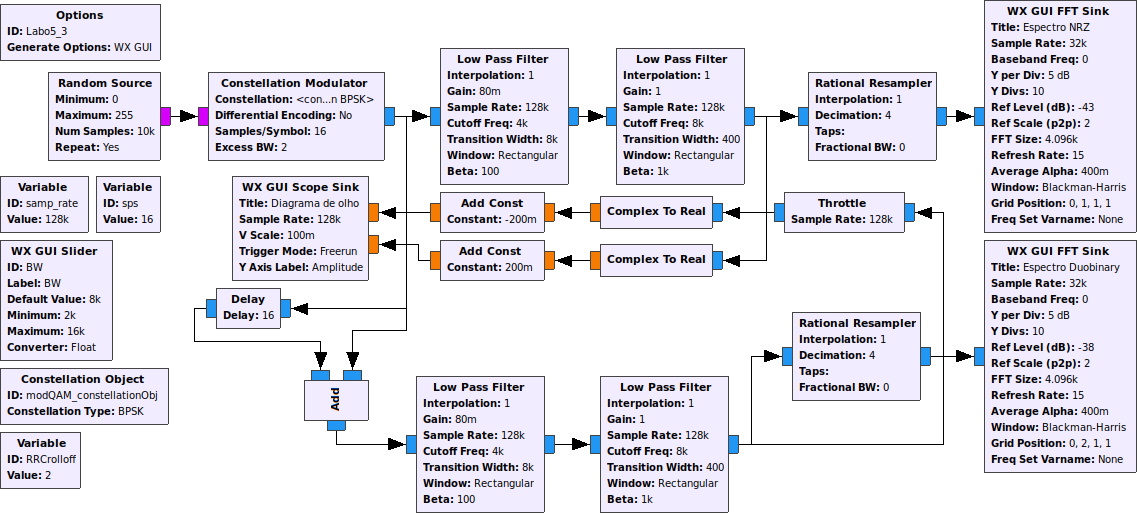
\includegraphics[width=\textwidth]{Figuras/Labo5-3}
        \caption{Diagrama de blocos de sistema de transmissão QPSK com pulsos NRZ e com pulsos duobinários.} 
        \label{fig:GRC_5-3}
    \end{figure}
  \item Execute o experimento e responda as questões propostas na Folha de Respostas.
\end{enumerate}

\subsection{Experimento 4 -- Modulação digital}

O objetivo deste experimento é mostrar o conceito de um receptor FM usando deteção por inclinação.

\begin{enumerate}
    \item  Abra o arquivo \textbf{Labo5-4.grc} disponibilizado pelo professor. A Figura \ref{fig:GRC_5-4} ilustra o diagrama deste experimento. Ele consiste de um sistema de transmissão digital modulada, que permite monitorar as constelações dos sinais transmitidos e recebidos, o espectro do sinal recebido, além da taxa de erro de bits (BER) e da relação sinal-ruído (SNR) obtidas na recepção.
    \begin{figure}[htb]
        \centering
        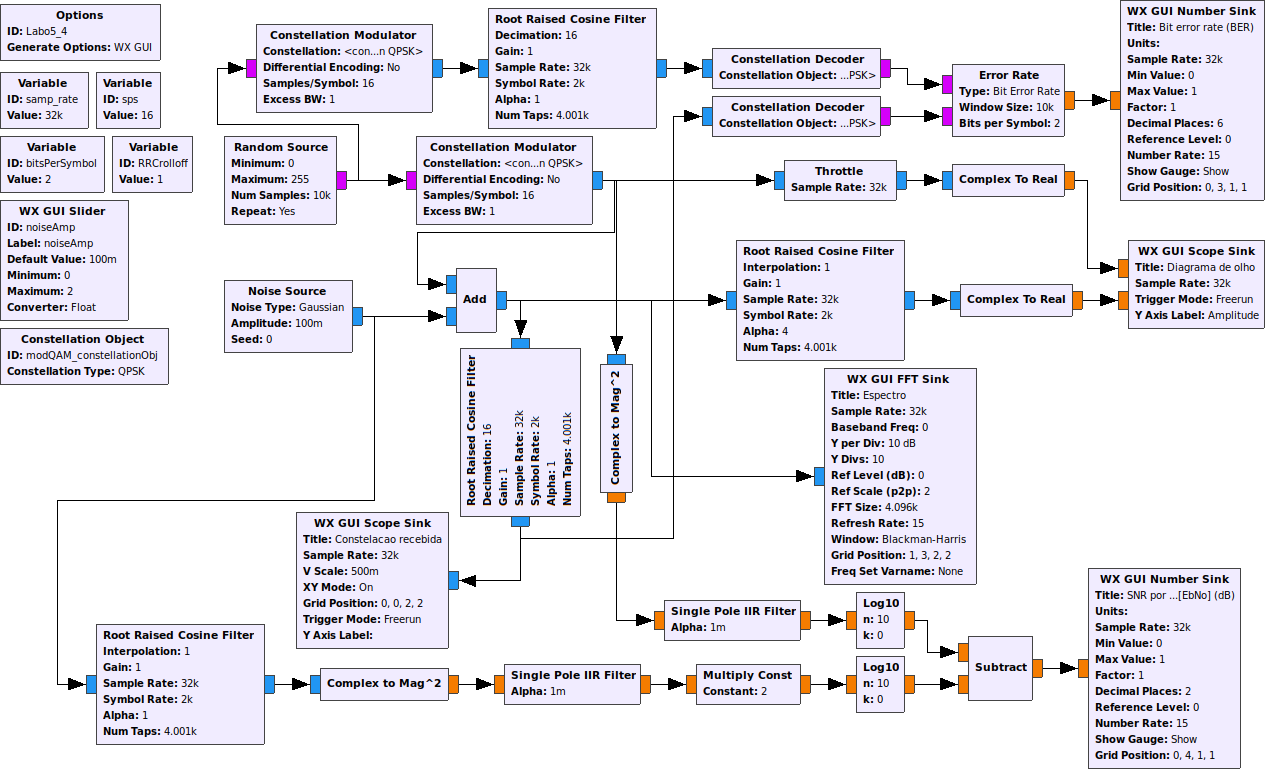
\includegraphics[width=0.8\textwidth]{Figuras/Labo5-4}
        \caption{Diagrama de blocos de sistema de transmissão digital modulada.} 
        \label{fig:GRC_5-4}
    \end{figure}
  \item Execute o experimento e responda as questões propostas na Folha de Respostas.
\end{enumerate}


\clearpage
\newpage \pagenumbering{arabic}

\noindent 
\includegraphics[height=2cm]{../Figuras/UFCGLogo} \hfill
\begin{minipage}{.66\textwidth} \large \centering \vspace{-1.8cm}
    Universidade Federal de Campina Grande -- UFCG \\
    Unidade Acadêmica de Engenharia Elétrica -- UAEE \\
    Curso de Graduação em Engenharia Elétrica
\end{minipage}
\hfill 
\includegraphics[height=2cm]{../Figuras/DEELogo} \\[12pt]

\noindent
\begin{tabular*}{\textwidth}{l @{\extracolsep{\fill}} r @{\extracolsep{6pt}} l}
    \textbf{\disciplina} && \\
    Período \periodo && \\
    \textbf{\avaliacao\ -- Folha de Respostas} && \\
    Tema(s): \tema && \\
    Professor(es): \professor && \\[12pt]
    \textbf{Aluno:} \hrulefill && \textbf{Data:} \makebox[3cm]{\hrulefill}
\end{tabular*}
\noindent\rule[2ex]{\textwidth}{2pt}

\section*{Experimento 1 -- Diagrama de olho}

\begin{questions}
    \question Observe o diagrama de olho desenhado para o sinal 2-PAM recebido sob baixo ruído (SNR de 30~dB). Esboce esse diagrama e identifique suas componentes (período, amplitude de abertura, etc.).
    \makeemptybox{5cm}
    
    \question Aumente o nível de ruído até obter SNR de $\approx$20~dB. Qual o efeito observado no diagrama de olho?
    \fillwithlines{0.75in}
    
    \question Retorne a SNR para 30~dB. Em seguida, altere a variável M de 2 para 4, para mudar a modulação de 2-PAM para 4-PAM. Explique porque o diagrama de olho agora apresenta mais níveis de amplitude e o que cada nível representa.
    \fillwithlines{1in}
\end{questions}

\section*{Experimento 2 -- Equalização}

\begin{questions}
    \question Descreva o que acontece com o diagrama de olho na saída do canal à medida em que distâncias de propagação aumentam. Justifique.
    \fillwithlines{0.75in}
    \question Descreva o que aconteceu com o diagrama de olho do sinal após o emprego do equalizador projetado. Justifique.
    \fillwithlines{0.75in}
    \question Que arranjo de blocos permite a equalização da dispersão cromática para uma distância de 4000~km com um filtro projetado para compensar uma distância 2000~km? Teste-o na simulação. Funciona? Desenhe o arranjo abaixo. (Vide questão 3 da preparação)
    \makeemptybox{4cm}  
\end{questions}

\section*{Experimento 3 -- Código duobinário}

\begin{questions}
    \question Considerando o canal com largura de faixa de 2~kHz, como inicialmente configurado, observe os espectros dos sinais e os diagramas de olho para o uso de pulsos NRZ (em azul) e de pulsos duobinários (em verde). Observe que ambos os diagramas de olho apresentam igual nível de abertura do olho. Agora, reduza a largura de faixa do canal para 1~kHz depois para 0.8~kHz e observe os diagramas de olho resultantes. Com base no observado, descreva as vantagens ou desvantagens do uso de pulsos duobinários em sistemas com restrição de largura de faixa em relação a pulsos NRZ.
    \fillwithlines{0.75in}
\end{questions}

\section*{Experimento 4 -- Modulação digital}

\begin{questions}
    \question Qual a SNR$_b$ (SNR por bit) e a BER observadas? Varie o nível de ruído do canal através da régua deslizante. O que ocorre com a SNR$_b$ e a BER quando o nível de ruído é aumentado ou diminuído.
    \fillwithlines{0.75in}
    
    \question A que nível de SNR$_b$ obtém-se uma BER de aproximadamente $10^{-4}$, ou seja, um erro em cada 10~kbits transmitidos?
    \fillwithlines{0.25in}
    
    \question Altere a variável M de 4 para 16 de forma a gerar o formato de modulação 16-QAM. Para esta modulação, a que nível de SNR$_b$ obtém-se uma BER de aproximadamente $10^{-4}$? Compare com o valor obtido para 4-QAM e apresente razões para a diferença. Repita o mesmo para M = 64.
    
    \fillwithlines{1in}
\end{questions}

\end{document}
